\documentclass[10pt,aspectratio=169,serif]{beamer}

\usepackage[fontset=none, scheme=plain]{ctex}
\IfFontExistsTF{Songti SC}{%
	\setCJKmainfont{Songti SC}[AutoFakeSlant=0.2]%
	\setCJKsansfont{Songti SC}[AutoFakeSlant=0.2]%
}{%
	\setCJKmainfont{FandolSong-Regular}[Extension=.otf,BoldFont=FandolSong-Bold,AutoFakeSlant=0.2]%
	\setCJKsansfont{FandolSong-Regular}[Extension=.otf,BoldFont=FandolSong-Bold]%
}
\usepackage{amsmath,amssymb,graphicx,tikz,booktabs,multicol,calligra}
\usepackage{pgfplots}
\pgfplotsset{compat=1.18}
\usepackage{tcolorbox}
\tcbuselibrary{skins}
\usepackage{XyygU}
\usepackage{caption}
\captionsetup[figure]{name=图,labelsep=period}

\usetikzlibrary{arrows.meta,positioning,calc}

\setlength{\abovedisplayskip}{0pt plus 2pt minus 2pt}
\setlength{\belowdisplayskip}{0pt plus 2pt minus 2pt}

\title[复习参考题4]{复习参考题 4：指数函数与对数函数}
\subtitle{复习巩固 \& 综合运用 \& 拓广探索}
\author{}
\institute{}
\date{2026-10-16}

\begin{document}

\begin{frame}
  \titlepage
\end{frame}

% ============================================================
% 第1题 选择题
% ============================================================
\begin{frame}[t]{第1题：选择题（指数/对数图象）}
\textbf{1.} 选择题：
\begin{enumerate}[(1)]
  \item 函数 $y=-2^{-x}$ 与 $y=2^{x}$ 的图象（\quad）。\\
  (A) 关于 $x$ 轴对称\qquad (B) 关于 $y$ 轴对称\\
  (C) 关于原点对称\qquad (D) 关于直线 $y=x$ 对称
  \item 图(1)中，\textcircled{1}\textcircled{2}\textcircled{3}\textcircled{4} 不属于 $y=2^{x},y=6^{x},y=(\tfrac12)^{x}$ 的是（\quad）。
  \item 图(2)中，\textcircled{1}\textcircled{2}\textcircled{3}\textcircled{4} 不属于 $y=\log_{1/2}x,y=\log_{1/3}x,y=\log_{2}x$ 的是（\quad）。
\end{enumerate}
\end{frame}

\begin{frame}[t]{第1题 解答}
\begin{tcolorbox}[colback=orange!10,colframe=orange,title=\textbf{解}]
\textbf{(1)} $y=-2^{-x}=-(\tfrac12)^{x}$。点 $(x,2^{x})$ 在 $y=2^{x}$ 上，对应点 $(-x,-2^{x})$ 在 $y=-2^{-x}$ 上，即关于原点对称。\textbf{选 C}。
\smallskip
\textbf{(2)} $y=2^{x},y=6^{x}$ 为递增指数函数，$y=(\tfrac12)^{x}$ 为递减指数函数。图(1)中 \textcircled{1} 为 $y=(\tfrac12)^{x}$，\textcircled{3}\textcircled{4} 为两个递增指数函数，\textcircled{2} 为另一个递减指数函数，不属于所给三者。\textbf{选 B}。
\smallskip
\textbf{(3)} $y=\log_{1/2}x,y=\log_{1/3}x$ 递减，$y=\log_{2}x$ 递增。图(2)中 \textcircled{1}\textcircled{2} 为两条递减对数曲线，\textcircled{4} 为 $y=\log_{2}x$，\textcircled{3} 为另一条递增对数曲线（如 $y=\log_{3}x$），不属于所给三者。\textbf{选 C}。
\end{tcolorbox}
\end{frame}

% ============================================================
% 第2题 比较大小
% ============================================================
\begin{frame}[t]{第2题：比较大小}
\textbf{2.} 用 ``$<$''、``$>$''、``$=$'' 填空：
\begin{enumerate}[(1)]
  \item $e^{0.8}$ \underline{\quad} $0.8^{e}$；
  \item $2^{a+1}$ \underline{\quad} $3^{a}\ (a>2)$；
  \item $a^{0.2}$ \underline{\quad} $a^{0.3}\ (0<a<1)$；
  \item $\lg e$ \underline{\quad} $\ln 0.8$；
  \item $\log_{2}3$ \underline{\quad} $\log_{3}2$；
  \item $\log_{a}0.2$ \underline{\quad} $\log_{a}0.3\ (a>1)$。
\end{enumerate}
\end{frame}

\begin{frame}[t]{第2题 解答}
\begin{tcolorbox}[colback=orange!10,colframe=orange,title=\textbf{解}]
\begin{enumerate}[(1)]
  \item $e^{0.8}\approx 2.22>1$，$0.8^{e}\approx 0.55<1$，故 $e^{0.8}\ \alert{>}\ 0.8^{e}$；
  \item $a>2$ 时 $\left(\tfrac{2}{3}\right)^{a}<\tfrac{4}{9}<\tfrac12$，故 $2^{a+1}=2\cdot 2^{a}<3^{a}$，填 $\alert{<}$；
  \item $0<a<1$ 时 $a^{x}$ 递减，$0.2<0.3$，故 $a^{0.2}\ \alert{>}\ a^{0.3}$；
  \item $\lg e>0$，$\ln 0.8<0$，故 $\lg e\ \alert{>}\ \ln 0.8$；
  \item $\log_{2}3>1$，$\log_{3}2<1$，故 $\log_{2}3\ \alert{>}\ \log_{3}2$；
  \item $a>1$ 时 $\log_{a}x$ 递增，$0.2<0.3$，故 $\log_{a}0.2\ \alert{<}\ \log_{a}0.3$。
\end{enumerate}
\end{tcolorbox}
\end{frame}

% ============================================================
% 第3题 二分法
% ============================================================
\begin{frame}[t]{第3题：二分法求根}
\textbf{3.} 借助信息技术，用二分法：
\begin{enumerate}[(1)]
  \item 求方程 $2x^{3}-4x^{2}-3x+1=0$ 的最大的根（精确度为 $0.01$）；
  \item 求函数 $f(x)=\lg x$ 和 $g(x)=\dfrac{1}{x}$ 交点的横坐标（精确度为 $0.1$）。
\end{enumerate}
\end{frame}

\begin{frame}[t]{第3题 解答 (1)}
\begin{tcolorbox}[colback=orange!10,colframe=orange,title=\textbf{解 (1)}]
令 $f(x)=2x^{3}-4x^{2}-3x+1$。$f(2)=-5<0$，$f(3)=10>0$，最大根在 $(2,3)$。
\smallskip
\begin{enumerate}
  \item $c=2.5$，$f(2.5)=-0.25<0$ $\Rightarrow (2.5,3)$；
  \item $c=2.75$，$f(2.75)\approx 4.09>0$ $\Rightarrow (2.5,2.75)$；
  \item $c=2.625$，$f(2.625)\approx 1.74>0$ $\Rightarrow (2.5,2.625)$；
  \item $c=2.5625$，$f\approx 0.70>0$ $\Rightarrow (2.5,2.5625)$；
  \item $c=2.53125$，$f\approx 0.24>0$ $\Rightarrow (2.5,2.53125)$；
  \item $c=2.5156$，$f\approx 0.003\approx 0$。
\end{enumerate}
\textbf{最大根约为 } $\alert{x\approx 2.51}$。
\end{tcolorbox}
\end{frame}

\begin{frame}[t]{第3题 解答 (2)}
\begin{tcolorbox}[colback=orange!10,colframe=orange,title=\textbf{解 (2)}]
交点满足 $\lg x=\dfrac{1}{x}$，即 $h(x)=x\lg x-1=0$。
\smallskip
$h(2)\approx -0.398<0$，$h(3)\approx 0.432>0$，根在 $(2,3)$。
\begin{enumerate}
  \item $c=2.5$，$h(2.5)\approx -0.005\approx 0$；
  \item $c=2.75$，$h\approx 0.208>0$ $\Rightarrow (2.5,2.75)$；
  \item $c=2.625$，$h\approx 0.100>0$ $\Rightarrow (2.5,2.625)$；
  \item $c=2.5625$，$h\approx 0.047>0$ $\Rightarrow (2.5,2.5625)$。
\end{enumerate}
$|2.5625-2.5|=0.0625<0.1$。
\textbf{交点横坐标约为 } $\alert{x\approx 2.53}$。
\end{tcolorbox}
\end{frame}

% ============================================================
% 第4题 分段函数解的个数
% ============================================================
\begin{frame}[t]{第4题：分段方程解的个数}
\textbf{4.} 已知函数
\[
f(x)=\begin{cases}
x^{2}+2x-3, & x\le 0,\\
-2+\ln x, & x>0.
\end{cases}
\]
求使方程 $f(x)=k$ 的实数解个数分别为 $1,2,3$ 时 $k$ 的相应取值范围。
\end{frame}

\begin{frame}[t]{第4题 解答}
\begin{tcolorbox}[colback=orange!10,colframe=orange,title=\textbf{解}]
\textbf{左支（$x\le 0$）：} $y=(x+1)^{2}-4$，顶点 $(-1,-4)$，$x=0$ 时 $y=-3$。
\begin{itemize}
  \item $k>-3$：左支 $1$ 解；
  \item $k=-3$：左支 $2$ 解（$x=0,-2$）；
  \item $-4<k<-3$：左支 $2$ 解；
  \item $k=-4$：左支 $1$ 解（$x=-1$，二重）；
  \item $k<-4$：左支 $0$ 解。
\end{itemize}
\textbf{右支（$x>0$）：} $y=-2+\ln x$ 严格递增，任意 $k$ 都有 $1$ 解。
\smallskip
\textbf{合计：}
\begin{itemize}
  \item \textbf{1 解：}$\alert{k<-4}$；
  \item \textbf{2 解：}$\alert{k=-4\text{ 或 }k>-3}$；
  \item \textbf{3 解：}$\alert{-4<k\le -3}$。
\end{itemize}
\end{tcolorbox}
\end{frame}

% ============================================================
% 第5题 选择题
% ============================================================
\begin{frame}[t]{第5题：选择题}
\textbf{5.} 选择题：
\begin{enumerate}[(1)]
  \item 集合 $A=\{y\mid y=\log_{2}x,\ x>1\}$，$B=\{y\mid y=\tfrac{1}{2^{x}},\ x>1\}$，则 $A\cap B=$（\quad）。\\
  (A) $\{y\mid 0<y<\tfrac12\}$\quad (B) $\{y\mid 0<y<1\}$\\
  (C) $\{y\mid \tfrac12<y<1\}$\quad (D) $\varnothing$
  \item $f(x)=|\lg x|$，$a=f(\tfrac14)$，$b=f(\tfrac13)$，$c=f(2)$，则（\quad）。\\
  (A) $a<b<c$\quad (B) $b<c<a$\quad (C) $c<a<b$\quad (D) $c<b<a$
  \item $f(x)=2^{x}+x$，$g(x)=\log_{2}x+x$，$h(x)=x^{3}+x$ 的零点分别为 $a,b,c$，则 $a,b,c$ 大小顺序为（\quad）。\\
  (A) $a>b>c$\quad (B) $b>c>a$\quad (C) $c>a>b$\quad (D) $b>a>c$
\end{enumerate}
\end{frame}

\begin{frame}[t]{第5题 解答}
\begin{tcolorbox}[colback=orange!10,colframe=orange,title=\textbf{解}]
\textbf{(1)} $A=\{y\mid y>0\}$，$B=\{y\mid 0<y<\tfrac12\}$。$A\cap B=\{y\mid 0<y<\tfrac12\}$。\textbf{选 A}。
\smallskip
\textbf{(2)} $a=|\lg\tfrac14|=\lg 4\approx 0.60$，$b=|\lg\tfrac13|=\lg 3\approx 0.48$，$c=|\lg 2|=\lg 2\approx 0.30$。故 $c<b<a$。\textbf{选 D}。
\smallskip
\textbf{(3)} $f(a)=0\Rightarrow 2^{a}+a=0$，$2^{a}>0$ 故 $a<0$；$h(c)=0\Rightarrow c^{3}+c=0\Rightarrow c=0$；$g(b)=0\Rightarrow \log_{2}b+b=0$，$0<b<1$。故 $a<c<b$，即 $b>c>a$。\textbf{选 B}。
\end{tcolorbox}
\end{frame}

% ============================================================
% 第6题 证明
% ============================================================
\begin{frame}[t]{第6题：双曲函数恒等式}
\textbf{6.} 设 $f(x)=\dfrac{e^{x}-e^{-x}}{2}$，$g(x)=\dfrac{e^{x}+e^{-x}}{2}$，求证：
\begin{enumerate}[(1)]
  \item $[g(x)]^{2}-[f(x)]^{2}=1$；
  \item $f(2x)=2f(x)g(x)$；
  \item $g(2x)=[g(x)]^{2}+[f(x)]^{2}$。
\end{enumerate}
\end{frame}

\begin{frame}[t]{第6题 证明}
\begin{tcolorbox}[colback=orange!10,colframe=orange,title=\textbf{证明}]
\textbf{(1)}
\[
g^{2}-f^{2}=\frac{(e^{x}+e^{-x})^{2}-(e^{x}-e^{-x})^{2}}{4}
=\frac{4}{4}=1.
\]
\textbf{(2)}
\[
2fg=2\cdot\frac{e^{x}-e^{-x}}{2}\cdot\frac{e^{x}+e^{-x}}{2}
=\frac{e^{2x}-e^{-2x}}{2}=f(2x).
\]
\textbf{(3)}
\[
g^{2}+f^{2}=\frac{(e^{x}+e^{-x})^{2}+(e^{x}-e^{-x})^{2}}{4}
=\frac{2(e^{2x}+e^{-2x})}{4}
=\frac{e^{2x}+e^{-2x}}{2}=g(2x).
\]
\end{tcolorbox}
\end{frame}

% ============================================================
% 第7题 二次函数顶点
% ============================================================
\begin{frame}[t]{第7题：二次函数顶点横坐标范围}
\textbf{7.} 指数函数 $y=\left(\dfrac{b}{a}\right)^{x}$ 的图象如图所示（递减），求二次函数 $y=ax^{2}+bx$ 图象顶点的横坐标的取值范围。
\smallskip
\begin{center}
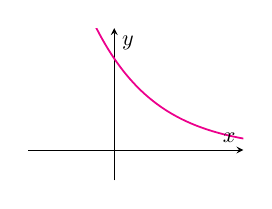
\begin{tikzpicture}[scale=0.8]
\begin{axis}[width=5cm,height=4cm,axis lines=middle,xtick=\empty,ytick=\empty,
  xlabel=$x$,ylabel=$y$,xmin=-2,xmax=3,ymin=-1,ymax=4]
\addplot[thick,magenta,domain=-0.5:3,samples=50]{(1/2)^x*3};
\end{axis}
\end{tikzpicture}
\end{center}
\end{frame}

\begin{frame}[t]{第7题 解答}
\begin{tcolorbox}[colback=orange!10,colframe=orange,title=\textbf{解}]
$y=\left(\dfrac{b}{a}\right)^{x}$ 递减，故 $0<\dfrac{b}{a}<1$。
\smallskip
二次函数 $y=ax^{2}+bx$ 顶点横坐标：
\[
x_{v}=-\frac{b}{2a}=-\frac{1}{2}\cdot\frac{b}{a}.
\]
由 $0<\dfrac{b}{a}<1$，得：
\[
0<\frac{1}{2}\cdot\frac{b}{a}<\frac12,
\]
两边乘 $-1$：
\[
\alert{-\frac12<x_{v}<0}.
\]
\textbf{顶点横坐标的取值范围为 } $\left(-\dfrac12,\ 0\right)$。
\end{tcolorbox}
\end{frame}

% ============================================================
% 第8题 锶90
% ============================================================
\begin{frame}[t]{第8题：切尔诺贝利锶90}
\textbf{8.} 1986 年切尔诺贝利核电站爆炸，主要核污染物锶 90 每年衰减率为 $2.47\%$。专家估计要完全消除事故影响至少需 $800$ 年，到那时原有的锶 90 还剩百分之几？
\end{frame}

\begin{frame}[t]{第8题 解答}
\begin{tcolorbox}[colback=orange!10,colframe=orange,title=\textbf{解}]
剩余量模型：$y=(1-0.0247)^{t}=0.9753^{t}$。
$t=800$：
\[
y=0.9753^{800}.
\]
取对数：
\[
\ln y=800\cdot\ln 0.9753\approx 800\times(-0.02501)\approx -20.01.
\]
\[
y=e^{-20.01}\approx 2.0\times 10^{-9}.
\]
换算为百分比：
\[
y\times 100\%\approx 2.0\times 10^{-7}\%\approx 0.0000002\%.
\]
\textbf{800 年后锶 90 剩余约 } $\alert{2\times 10^{-7}\%}$\textbf{，几乎为零。}
\end{tcolorbox}
\end{frame}

% ============================================================
% 第9题 废气过滤
% ============================================================
\begin{frame}[t]{第9题：废气过滤模型}
\textbf{9.} 过滤过程中废气污染物含量 $P$（mg/L）与时间 $t$（h）关系 $P=P_{0}e^{-kt}$。前 $5$ h 消除了 $10\%$ 污染物。
\begin{enumerate}[(1)]
  \item $10$ h 后还剩百分之几污染物？
  \item 污染物减少 $50\%$ 需要多少时间（精确到 $1$ h）？
  \item 画出 $P$ 关于 $t$ 的函数图象。
\end{enumerate}
\end{frame}

\begin{frame}[t]{第9题 解答}
\begin{tcolorbox}[colback=orange!10,colframe=orange,title=\textbf{解}]
$t=5$ 时 $P=0.9P_{0}$：
\[
0.9=e^{-5k}\Rightarrow k=-\frac{\ln 0.9}{5}\approx 0.02107.
\]
\textbf{(1)} $t=10$：
\[
P=P_{0}e^{-0.02107\times 10}=P_{0}e^{-0.2107}\approx 0.81P_{0}.
\]
即剩余 $\alert{81\%}$。
\smallskip
\textbf{(2)} $P=0.5P_{0}$：
\[
e^{-kt}=0.5\Rightarrow t=\frac{\ln 2}{k}=\frac{0.6931}{0.02107}\approx \alert{33\ \text{h}}.
\]
\smallskip
\textbf{(3)} 图象为指数衰减曲线：从 $P_{0}$ 单调递减，逐渐趋近于 $0$。
\end{tcolorbox}
\end{frame}

% ============================================================
% 第10题 冷却模型
% ============================================================
\begin{frame}[t]{第10题：牛顿冷却模型}
\textbf{10.} 物体冷却公式 $\theta=\theta_{0}+(\theta_{1}-\theta_{0})e^{-kt}$。现有 $62\,^{\circ}\text{C}$ 物体放在 $15\,^{\circ}\text{C}$ 空气中，$1$ min 后温度为 $52\,^{\circ}\text{C}$。
\begin{enumerate}[(1)]
  \item 求 $k$（精确到 $0.01$）；
  \item 物体降到 $42\,^{\circ}\text{C}$、$32\,^{\circ}\text{C}$ 各需多少时间（精确到 $0.1$ min）？
\end{enumerate}
\end{frame}

\begin{frame}[t]{第10题 解答}
\begin{tcolorbox}[colback=orange!10,colframe=orange,title=\textbf{解}]
$\theta_{1}=62$，$\theta_{0}=15$。$t=1$ 时 $\theta=52$：
\[
52=15+47e^{-k}\Rightarrow e^{-k}=\frac{37}{47}\approx 0.787.
\]
\textbf{(1)} $k=-\ln 0.787\approx \alert{0.24}$。
\smallskip
\textbf{(2)} $\theta=42$：
\[
42=15+47e^{-0.24t}\Rightarrow e^{-0.24t}=\frac{27}{47}\approx 0.574
\Rightarrow t\approx \alert{2.3\ \text{min}}.
\]
$\theta=32$：
\[
e^{-0.24t}=\frac{17}{47}\approx 0.362
\Rightarrow t\approx \alert{4.3\ \text{min}}.
\]
\end{tcolorbox}
\end{frame}

% ============================================================
% 第11题 对数函数奇偶性
% ============================================================
\begin{frame}[t]{第11题：对数函数的奇偶性}
\textbf{11.} 已知 $f(x)=\log_{a}(x+1)$，$g(x)=\log_{a}(1-x)$（$a>0$，$a\ne 1$）。
\begin{enumerate}[(1)]
  \item 求函数 $f(x)+g(x)$ 的定义域；
  \item 判断 $f(x)+g(x)$ 的奇偶性，并说明理由。
\end{enumerate}
\end{frame}

\begin{frame}[t]{第11题 解答}
\begin{tcolorbox}[colback=orange!10,colframe=orange,title=\textbf{解}]
\textbf{(1)}
\[
f(x)+g(x)=\log_{a}(x+1)+\log_{a}(1-x)=\log_{a}(1-x^{2}).
\]
需 $x+1>0$ 且 $1-x>0$，即 $-1<x<1$。
\textbf{定义域：}$\alert{(-1,1)}$。
\smallskip
\textbf{(2)} 设 $h(x)=f(x)+g(x)=\log_{a}(1-x^{2})$。
\[
h(-x)=\log_{a}(1-(-x)^{2})=\log_{a}(1-x^{2})=h(x).
\]
\textbf{故 $f(x)+g(x)$ 为 }$\alert{\text{偶函数}}$。
\end{tcolorbox}
\end{frame}

% ============================================================
% 第12题 f(x) = a - 2/(2^x+1)
% ============================================================
\begin{frame}[t]{第12题：探究函数单调性与奇偶性}
\textbf{12.} 对于函数 $f(x)=a-\dfrac{2}{2^{x}+1}$（$a\in\mathbf{R}$）。
\begin{enumerate}[(1)]
  \item 探索函数 $f(x)$ 的单调性；
  \item 是否存在实数 $a$ 使 $f(x)$ 为奇函数？
\end{enumerate}
\end{frame}

\begin{frame}[t]{第12题 解答}
\begin{tcolorbox}[colback=orange!10,colframe=orange,title=\textbf{解}]
\textbf{(1)} $2^{x}$ 在 $\mathbf{R}$ 上严格递增，故 $\dfrac{2}{2^{x}+1}$ 严格递减，从而
\[
f(x)=a-\frac{2}{2^{x}+1}
\]
在 $\mathbf{R}$ 上\alert{严格递增}。
\smallskip
\textbf{(2)} 若 $f(x)$ 为奇函数，则 $f(0)=0$：
\[
f(0)=a-\frac{2}{1+1}=a-1=0\Rightarrow a=1.
\]
验证：$f(x)=1-\dfrac{2}{2^{x}+1}=\dfrac{2^{x}-1}{2^{x}+1}$。
\[
f(-x)=\frac{2^{-x}-1}{2^{-x}+1}=\frac{1-2^{x}}{1+2^{x}}=-f(x).
\]
\textbf{存在 }$\alert{a=1}$\textbf{，使 $f(x)$ 为奇函数。}
\end{tcolorbox}
\end{frame}

% ============================================================
% 第13题 由图象求解析式
% ============================================================
\begin{frame}[t]{第13题：由图象写解析式}
\textbf{13.} 函数 $y=f(x)$ 图象由曲线段 $OA$ 和直线段 $AB$ 构成，$A(2,3)$，$B(5,0)$，$O$ 为原点。
\begin{enumerate}[(1)]
  \item 写出 $y=f(x)$ 的一个解析式；
  \item 提出一个能满足 $y=f(x)$ 变化规律的实际问题。
\end{enumerate}
\smallskip
\begin{center}
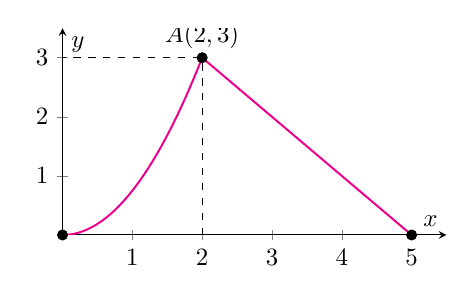
\begin{tikzpicture}[scale=0.9]
\begin{axis}[width=7cm,height=4.5cm,axis lines=middle,xtick={1,2,3,4,5},ytick={1,2,3},
  xlabel=$x$,ylabel=$y$,xmin=0,xmax=5.5,ymin=0,ymax=3.5]
\addplot[thick,magenta,domain=0:2,samples=50]{0.75*x^2};
\addplot[thick,magenta,domain=2:5,samples=2]{-x+5};
\addplot[only marks,mark=*,mark size=2pt] coordinates {(2,3)(5,0)(0,0)};
\node[above] at (axis cs:2,3) {$A(2,3)$};
\node[below right] at (axis cs:5,0) {$B(5,0)$};
\draw[dashed] (axis cs:2,0) -- (axis cs:2,3) -- (axis cs:0,3);
\end{axis}
\end{tikzpicture}
\end{center}
\end{frame}

\begin{frame}[t]{第13题 解答}
\begin{tcolorbox}[colback=orange!10,colframe=orange,title=\textbf{解}]
\textbf{(1)} 曲线段 $OA$ 过原点，设 $y=ax^{2}$，代入 $A(2,3)$：$3=4a\Rightarrow a=\tfrac34$。
直线段 $AB$ 斜率 $k=\dfrac{0-3}{5-2}=-1$，方程 $y-3=-(x-2)$，即 $y=-x+5$。
\[
f(x)=\begin{cases}
\dfrac34 x^{2}, & 0\le x\le 2,\\[4pt]
-x+5, & 2<x\le 5.
\end{cases}
\]
\smallskip
\textbf{(2) 实际问题示例：}一物体从原点出发前 $2$ 秒做加速运动（位移 $\propto t^{2}$），$2$ 秒后以恒定速度 $-1$（反向匀速）运动，第 $5$ 秒回到 $y=0$。
\end{tcolorbox}
\end{frame}

\begin{frame}[c]
  \begin{center}
    {\Huge\calligra Thanks!}
  \end{center}
\end{frame}

\end{document}
